\begin{frame}

\frametitle{I protagonisti}

\begin{block}{Lo Shellac}
\`E interessante conoscere alcune caratteristiche di questi oggetti:
\begin{itemize}
\item Diametro del disco = [8 in $\div$ 12 in]
\item Massima escursione possibile del solco $\sim$ 0.15 mm
\item Banda teorica = [30 Hz $\div$ 16000 Hz]
\item Banda reale = [500 Hz $\div$ 3500 Hz] 
\end{itemize}
Il segnale è inciso lateralemente $\Rightarrow$ Uno scanner è 
sufficente per ricavare le forme d'onda
\end{block}

\begin{block}{Lo scanner}
\begin{itemize}
\item Scanner \emph{flat}
\item Punto di illuminazione ideale diverso per ogni scanner
\item Risoluzione minima 1600 dpi non interpolati
\end{itemize}
\end{block}
\end{frame}

\begin{frame}
\frametitle{Shellac}
\begin{figure}
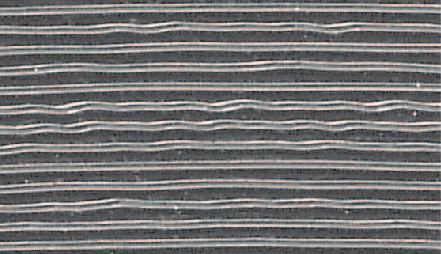
\includegraphics[width=\textwidth]{immagini/shellac-track.png}
\caption{Le tracce di uno \emph{shellac}}
\end{figure}
\end{frame}


